\documentclass[1p]{elsarticle_modified}
%\bibliographystyle{elsarticle-num}

%\usepackage[colorlinks]{hyperref}
%\usepackage{abbrmath_seonhwa} %\Abb, \Ascr, \Acal ,\Abf, \Afrak
\usepackage{amsfonts}
\usepackage{amssymb}
\usepackage{amsmath}
\usepackage{amsthm}
\usepackage{scalefnt}
\usepackage{amsbsy}
\usepackage{kotex}
\usepackage{caption}
\usepackage{subfig}
\usepackage{color}
\usepackage{graphicx}
\usepackage{xcolor} %% white, black, red, green, blue, cyan, magenta, yellow
\usepackage{float}
\usepackage{setspace}
\usepackage{hyperref}

\usepackage{tikz}
\usetikzlibrary{arrows}

\usepackage{multirow}
\usepackage{array} % fixed length table
\usepackage{hhline}

%%%%%%%%%%%%%%%%%%%%%
\makeatletter
\renewcommand*\env@matrix[1][\arraystretch]{%
	\edef\arraystretch{#1}%
	\hskip -\arraycolsep
	\let\@ifnextchar\new@ifnextchar
	\array{*\c@MaxMatrixCols c}}
\makeatother %https://tex.stackexchange.com/questions/14071/how-can-i-increase-the-line-spacing-in-a-matrix
%%%%%%%%%%%%%%%

\usepackage[normalem]{ulem}

\newcommand{\msout}[1]{\ifmmode\text{\sout{\ensuremath{#1}}}\else\sout{#1}\fi}
%SOURCE: \msout is \stkout macro in https://tex.stackexchange.com/questions/20609/strikeout-in-math-mode

\newcommand{\cancel}[1]{
	\ifmmode
	{\color{red}\msout{#1}}
	\else
	{\color{red}\sout{#1}}
	\fi
}

\newcommand{\add}[1]{
	{\color{blue}\uwave{#1}}
}

\newcommand{\replace}[2]{
	\ifmmode
	{\color{red}\msout{#1}}{\color{blue}\uwave{#2}}
	\else
	{\color{red}\sout{#1}}{\color{blue}\uwave{#2}}
	\fi
}

\newcommand{\Sol}{\mathcal{S}} %segment
\newcommand{\D}{D} %diagram
\newcommand{\A}{\mathcal{A}} %arc


%%%%%%%%%%%%%%%%%%%%%%%%%%%%%5 test

\def\sl{\operatorname{\textup{SL}}(2,\Cbb)}
\def\psl{\operatorname{\textup{PSL}}(2,\Cbb)}
\def\quan{\mkern 1mu \triangleright \mkern 1mu}

\theoremstyle{definition}
\newtheorem{thm}{Theorem}[section]
\newtheorem{prop}[thm]{Proposition}
\newtheorem{lem}[thm]{Lemma}
\newtheorem{ques}[thm]{Question}
\newtheorem{cor}[thm]{Corollary}
\newtheorem{defn}[thm]{Definition}
\newtheorem{exam}[thm]{Example}
\newtheorem{rmk}[thm]{Remark}
\newtheorem{alg}[thm]{Algorithm}

\newcommand{\I}{\sqrt{-1}}
\begin{document}

%\begin{frontmatter}
%
%\title{Boundary parabolic representations of knots up to 8 crossings}
%
%%% Group authors per affiliation:
%\author{Yunhi Cho} 
%\address{Department of Mathematics, University of Seoul, Seoul, Korea}
%\ead{yhcho@uos.ac.kr}
%
%
%\author{Seonhwa Kim} %\fnref{s_kim}}
%\address{Center for Geometry and Physics, Institute for Basic Science, Pohang, 37673, Korea}
%\ead{ryeona17@ibs.re.kr}
%
%\author{Hyuk Kim}
%\address{Department of Mathematical Sciences, Seoul National University, Seoul 08826, Korea}
%\ead{hyukkim@snu.ac.kr}
%
%\author{Seokbeom Yoon}
%\address{Department of Mathematical Sciences, Seoul National University, Seoul, 08826,  Korea}
%\ead{sbyoon15@snu.ac.kr}
%
%\begin{abstract}
%We find all boundary parabolic representation of knots up to 8 crossings.
%
%\end{abstract}
%\begin{keyword}
%    \MSC[2010] 57M25 
%\end{keyword}
%
%\end{frontmatter}

%\linenumbers
%\tableofcontents
%
\newcommand\colored[1]{\textcolor{white}{\rule[-0.35ex]{0.8em}{1.4ex}}\kern-0.8em\color{red} #1}%
%\newcommand\colored[1]{\textcolor{white}{ #1}\kern-2.17ex	\textcolor{white}{ #1}\kern-1.81ex	\textcolor{white}{ #1}\kern-2.15ex\color{red}#1	}

{\Large $\underline{12a_{0405}~(K12a_{0405})}$}

\setlength{\tabcolsep}{10pt}
\renewcommand{\arraystretch}{1.6}
\vspace{1cm}\begin{tabular}{m{100pt}>{\centering\arraybackslash}m{274pt}}
\multirow{5}{120pt}{
	\centering
	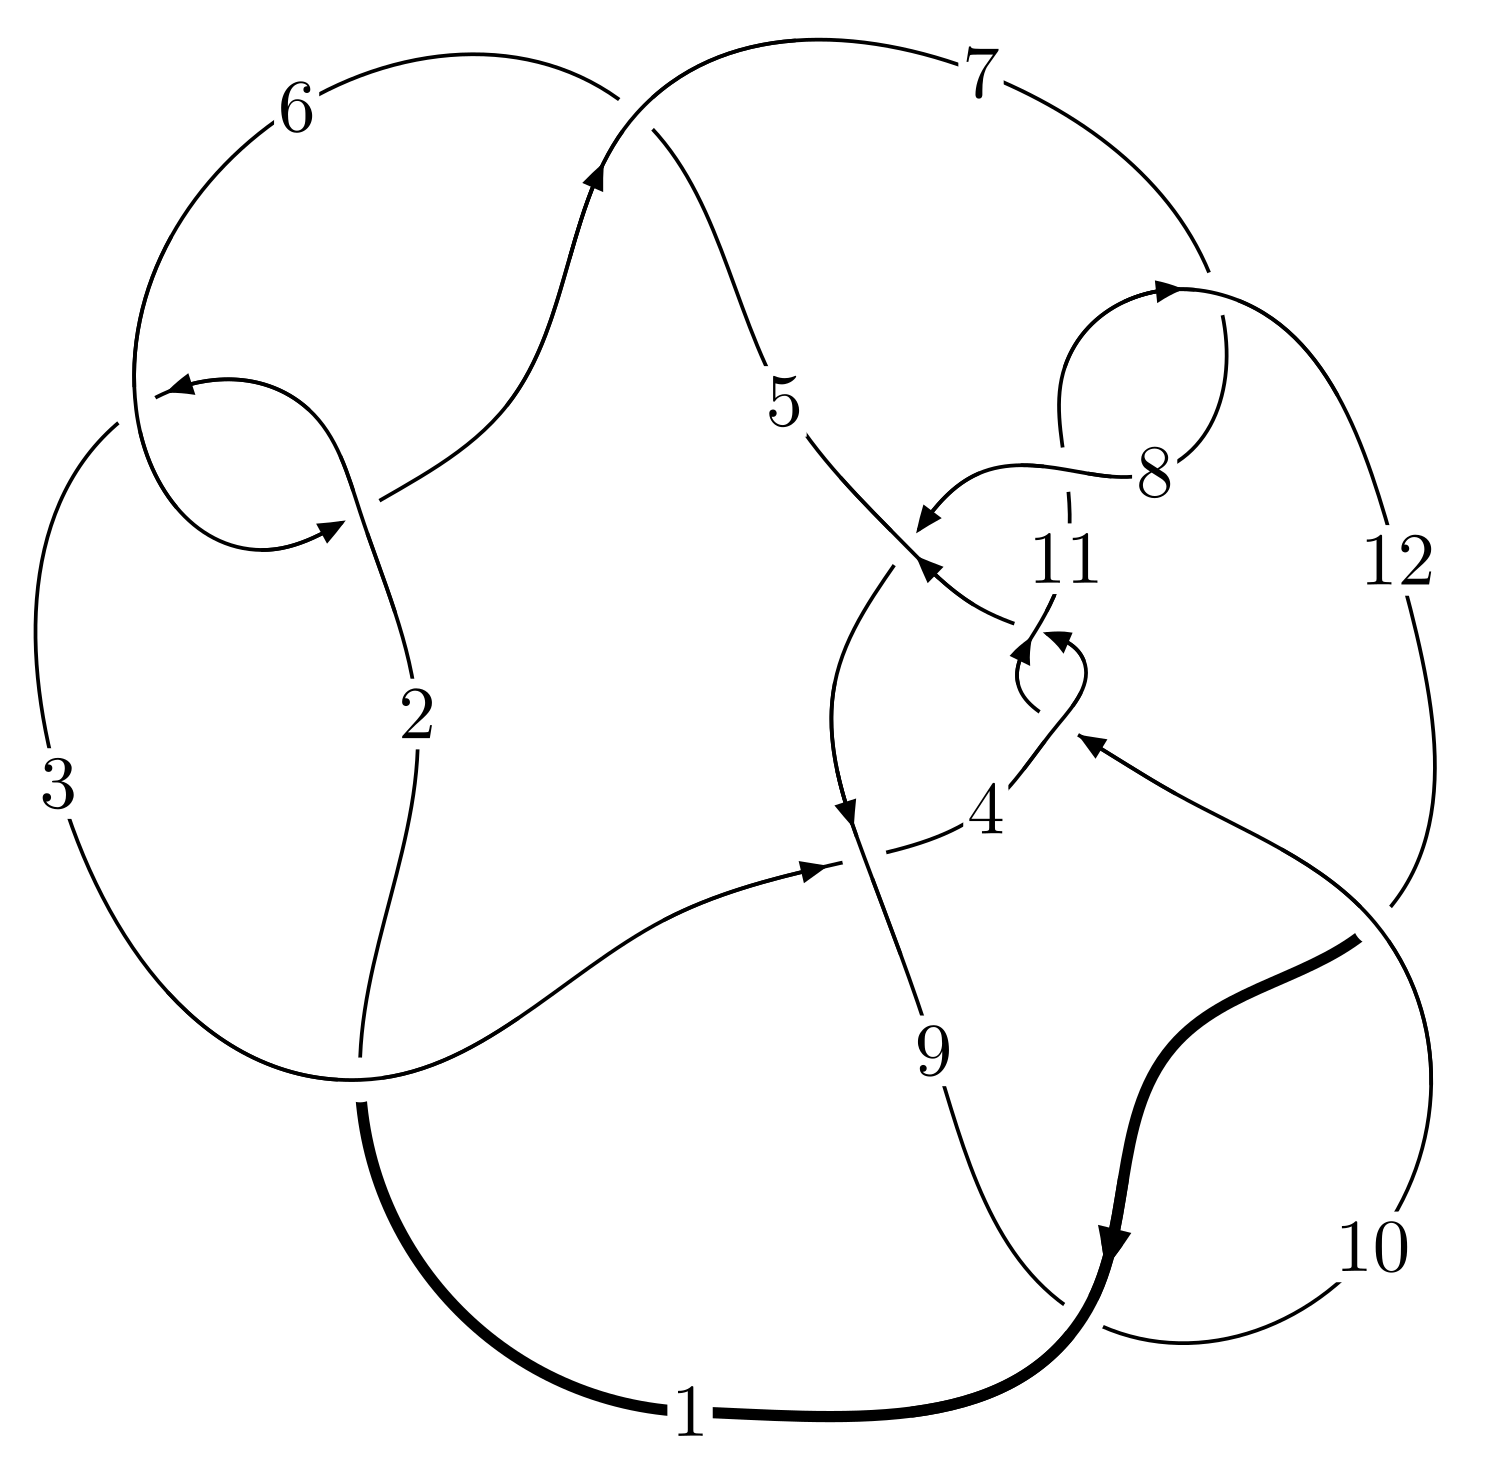
\includegraphics[width=112pt]{../../../GIT/diagram.site/Diagrams/png/1206_12a_0405.png}\\
\ \ \ A knot diagram\footnotemark}&
\allowdisplaybreaks
\textbf{Linearized knot diagam} \\
\cline{2-2}
 &
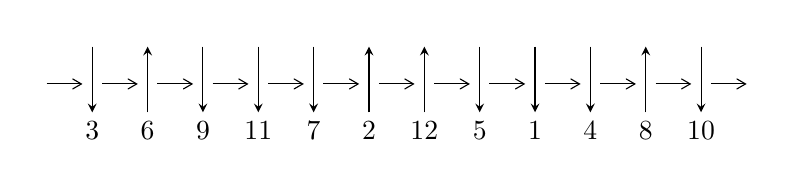
\begin{tikzpicture}[x=20pt, y=17pt]
	% nodes
	\node (C0) at (0, 0) {};
	\node (C1) at (1, 0) {};
	\node (C1U) at (1, +1) {};
	\node (C1D) at (1, -1) {3};

	\node (C2) at (2, 0) {};
	\node (C2U) at (2, +1) {};
	\node (C2D) at (2, -1) {6};

	\node (C3) at (3, 0) {};
	\node (C3U) at (3, +1) {};
	\node (C3D) at (3, -1) {9};

	\node (C4) at (4, 0) {};
	\node (C4U) at (4, +1) {};
	\node (C4D) at (4, -1) {11};

	\node (C5) at (5, 0) {};
	\node (C5U) at (5, +1) {};
	\node (C5D) at (5, -1) {7};

	\node (C6) at (6, 0) {};
	\node (C6U) at (6, +1) {};
	\node (C6D) at (6, -1) {2};

	\node (C7) at (7, 0) {};
	\node (C7U) at (7, +1) {};
	\node (C7D) at (7, -1) {12};

	\node (C8) at (8, 0) {};
	\node (C8U) at (8, +1) {};
	\node (C8D) at (8, -1) {5};

	\node (C9) at (9, 0) {};
	\node (C9U) at (9, +1) {};
	\node (C9D) at (9, -1) {1};

	\node (C10) at (10, 0) {};
	\node (C10U) at (10, +1) {};
	\node (C10D) at (10, -1) {4};

	\node (C11) at (11, 0) {};
	\node (C11U) at (11, +1) {};
	\node (C11D) at (11, -1) {8};

	\node (C12) at (12, 0) {};
	\node (C12U) at (12, +1) {};
	\node (C12D) at (12, -1) {10};
	\node (C13) at (13, 0) {};

	% arrows
	\draw[->,>={angle 60}]
	(C0) edge (C1) (C1) edge (C2) (C2) edge (C3) (C3) edge (C4) (C4) edge (C5) (C5) edge (C6) (C6) edge (C7) (C7) edge (C8) (C8) edge (C9) (C9) edge (C10) (C10) edge (C11) (C11) edge (C12) (C12) edge (C13) ;	\draw[->,>=stealth]
	(C1U) edge (C1D) (C2D) edge (C2U) (C3U) edge (C3D) (C4U) edge (C4D) (C5U) edge (C5D) (C6D) edge (C6U) (C7D) edge (C7U) (C8U) edge (C8D) (C9U) edge (C9D) (C10U) edge (C10D) (C11D) edge (C11U) (C12U) edge (C12D) ;
	\end{tikzpicture} \\
\hhline{~~} \\& 
\textbf{Solving Sequence} \\ \cline{2-2} 
 &
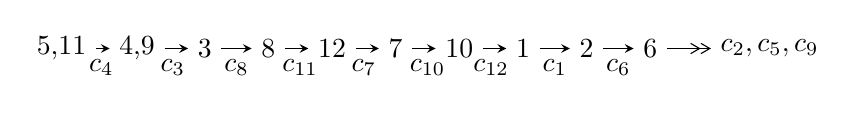
\begin{tikzpicture}[x=23pt, y=7pt]
	% node
	\node (A0) at (-1/8, 0) {5,11};
	\node (A1) at (17/16, 0) {4,9};
	\node (A2) at (17/8, 0) {3};
	\node (A3) at (25/8, 0) {8};
	\node (A4) at (33/8, 0) {12};
	\node (A5) at (41/8, 0) {7};
	\node (A6) at (49/8, 0) {10};
	\node (A7) at (57/8, 0) {1};
	\node (A8) at (65/8, 0) {2};
	\node (A9) at (73/8, 0) {6};
	\node (C1) at (1/2, -1) {$c_{4}$};
	\node (C2) at (13/8, -1) {$c_{3}$};
	\node (C3) at (21/8, -1) {$c_{8}$};
	\node (C4) at (29/8, -1) {$c_{11}$};
	\node (C5) at (37/8, -1) {$c_{7}$};
	\node (C6) at (45/8, -1) {$c_{10}$};
	\node (C7) at (53/8, -1) {$c_{12}$};
	\node (C8) at (61/8, -1) {$c_{1}$};
	\node (C9) at (69/8, -1) {$c_{6}$};
	\node (A10) at (11, 0) {$c_{2},c_{5},c_{9}$};

	% edge
	\draw[->,>=stealth]	
	(A0) edge (A1) (A1) edge (A2) (A2) edge (A3) (A3) edge (A4) (A4) edge (A5) (A5) edge (A6) (A6) edge (A7) (A7) edge (A8) (A8) edge (A9) ;
	\draw[->>,>={angle 60}]	
	(A9) edge (A10);
\end{tikzpicture} \\ 

\end{tabular} \\

\footnotetext{
The image of knot diagram is generated by the software ``\textbf{Draw programme}" developed by Andrew Bartholomew(\url{http://www.layer8.co.uk/maths/draw/index.htm\#Running-draw}), where we modified some parts for our purpose(\url{https://github.com/CATsTAILs/LinksPainter}).
}\phantom \\ \newline 
\centering \textbf{Ideals for irreducible components\footnotemark of $X_{\text{par}}$} 
 
\begin{align*}
I^u_{1}&=\langle 
1.74918\times10^{481} u^{118}+1.13087\times10^{480} u^{117}+\cdots+3.76444\times10^{482} b-5.51380\times10^{484},\\
\phantom{I^u_{1}}&\phantom{= \langle  }-1.88038\times10^{485} u^{118}-5.43563\times10^{485} u^{117}+\cdots+1.64393\times10^{486} a-1.41886\times10^{489},\\
\phantom{I^u_{1}}&\phantom{= \langle  }u^{119}+u^{118}+\cdots+4696 u-4367\rangle \\
I^u_{2}&=\langle 
134204 u^{23}-60433 u^{22}+\cdots+61210 b+20157,\;66179 u^{23}+20157 u^{22}+\cdots+61210 a+542412,\\
\phantom{I^u_{2}}&\phantom{= \langle  }u^{24}-12 u^{22}+\cdots+4 u+1\rangle \\
\\
\end{align*}
\raggedright * 2 irreducible components of $\dim_{\mathbb{C}}=0$, with total 143 representations.\\
\footnotetext{All coefficients of polynomials are rational numbers. But the coefficients are sometimes approximated in decimal forms when there is not enough margin.}
\newpage
\renewcommand{\arraystretch}{1}
\centering \section*{I. $I^u_{1}= \langle 1.75\times10^{481} u^{118}+1.13\times10^{480} u^{117}+\cdots+3.76\times10^{482} b-5.51\times10^{484},\;-1.88\times10^{485} u^{118}-5.44\times10^{485} u^{117}+\cdots+1.64\times10^{486} a-1.42\times10^{489},\;u^{119}+u^{118}+\cdots+4696 u-4367 \rangle$}
\flushleft \textbf{(i) Arc colorings}\\
\begin{tabular}{m{7pt} m{180pt} m{7pt} m{180pt} }
\flushright $a_{5}=$&$\begin{pmatrix}1\\0\end{pmatrix}$ \\
\flushright $a_{11}=$&$\begin{pmatrix}0\\u\end{pmatrix}$ \\
\flushright $a_{4}=$&$\begin{pmatrix}1\\- u^2\end{pmatrix}$ \\
\flushright $a_{9}=$&$\begin{pmatrix}0.114383 u^{118}+0.330648 u^{117}+\cdots-479.984 u+863.088\\-0.0464657 u^{118}-0.00300409 u^{117}+\cdots-357.274 u+146.471\end{pmatrix}$ \\
\flushright $a_{3}=$&$\begin{pmatrix}0.280271 u^{118}+0.0944427 u^{117}+\cdots+1600.16 u-614.771\\-0.263990 u^{118}-0.219179 u^{117}+\cdots-1351.59 u+269.403\end{pmatrix}$ \\
\flushright $a_{8}=$&$\begin{pmatrix}0.0679176 u^{118}+0.327644 u^{117}+\cdots-837.258 u+1009.56\\-0.0464657 u^{118}-0.00300409 u^{117}+\cdots-357.274 u+146.471\end{pmatrix}$ \\
\flushright $a_{12}=$&$\begin{pmatrix}0.0912004 u^{118}+0.106850 u^{117}+\cdots+7.29293 u+233.640\\0.0276670 u^{118}+0.278787 u^{117}+\cdots-959.393 u+957.198\end{pmatrix}$ \\
\flushright $a_{7}=$&$\begin{pmatrix}0.337154 u^{118}-0.160946 u^{117}+\cdots+3118.25 u-1883.61\\-0.00674423 u^{118}+0.0484890 u^{117}+\cdots-547.872 u+378.354\end{pmatrix}$ \\
\flushright $a_{10}=$&$\begin{pmatrix}u\\- u^3+u\end{pmatrix}$ \\
\flushright $a_{1}=$&$\begin{pmatrix}-0.0340855 u^{118}-0.210614 u^{117}+\cdots+513.977 u-581.351\\0.0715432 u^{118}+0.326265 u^{117}+\cdots-808.053 u+981.448\end{pmatrix}$ \\
\flushright $a_{2}=$&$\begin{pmatrix}-0.463324 u^{118}+0.0153182 u^{117}+\cdots-1875.61 u+975.097\\0.242350 u^{118}+0.159986 u^{117}+\cdots+913.110 u-158.555\end{pmatrix}$ \\
\flushright $a_{6}=$&$\begin{pmatrix}1.30834 u^{118}-0.0714837 u^{117}+\cdots+11338.6 u-5626.43\\-0.0561421 u^{118}-0.0515743 u^{117}+\cdots-1003.85 u+404.609\end{pmatrix}$\\&\end{tabular}
\flushleft \textbf{(ii) Obstruction class $= -1$}\\~\\
\flushleft \textbf{(iii) Cusp Shapes $= -0.522519 u^{118}+0.0348626 u^{117}+\cdots-3209.51 u+1608.47$}\\~\\
\newpage\renewcommand{\arraystretch}{1}
\flushleft \textbf{(iv) u-Polynomials at the component}\newline \\
\begin{tabular}{m{50pt}|m{274pt}}
Crossings & \hspace{64pt}u-Polynomials at each crossing \\
\hline $$\begin{aligned}c_{1},c_{5}\end{aligned}$$&$\begin{aligned}
&u^{119}+35 u^{118}+\cdots-7880 u-289
\end{aligned}$\\
\hline $$\begin{aligned}c_{2},c_{6}\end{aligned}$$&$\begin{aligned}
&u^{119}-5 u^{118}+\cdots+46 u+17
\end{aligned}$\\
\hline $$\begin{aligned}c_{3}\end{aligned}$$&$\begin{aligned}
&u^{119}+u^{118}+\cdots-1436808 u+659257
\end{aligned}$\\
\hline $$\begin{aligned}c_{4},c_{10}\end{aligned}$$&$\begin{aligned}
&u^{119}- u^{118}+\cdots+4696 u+4367
\end{aligned}$\\
\hline $$\begin{aligned}c_{7},c_{11}\end{aligned}$$&$\begin{aligned}
&u^{119}-3 u^{118}+\cdots+103202 u+32411
\end{aligned}$\\
\hline $$\begin{aligned}c_{8}\end{aligned}$$&$\begin{aligned}
&u^{119}-3 u^{118}+\cdots+64836 u-22801
\end{aligned}$\\
\hline $$\begin{aligned}c_{9},c_{12}\end{aligned}$$&$\begin{aligned}
&u^{119}-5 u^{118}+\cdots+3020 u+193
\end{aligned}$\\
\hline
\end{tabular}\\~\\
\newpage\renewcommand{\arraystretch}{1}
\flushleft \textbf{(v) Riley Polynomials at the component}\newline \\
\begin{tabular}{m{50pt}|m{274pt}}
Crossings & \hspace{64pt}Riley Polynomials at each crossing \\
\hline $$\begin{aligned}c_{1},c_{5}\end{aligned}$$&$\begin{aligned}
&y^{119}+107 y^{118}+\cdots+4464332 y-83521
\end{aligned}$\\
\hline $$\begin{aligned}c_{2},c_{6}\end{aligned}$$&$\begin{aligned}
&y^{119}+35 y^{118}+\cdots-7880 y-289
\end{aligned}$\\
\hline $$\begin{aligned}c_{3}\end{aligned}$$&$\begin{aligned}
&y^{119}+27 y^{118}+\cdots-1873336698762 y-434619792049
\end{aligned}$\\
\hline $$\begin{aligned}c_{4},c_{10}\end{aligned}$$&$\begin{aligned}
&y^{119}-89 y^{118}+\cdots+330458690 y-19070689
\end{aligned}$\\
\hline $$\begin{aligned}c_{7},c_{11}\end{aligned}$$&$\begin{aligned}
&y^{119}+77 y^{118}+\cdots-37961568944 y-1050472921
\end{aligned}$\\
\hline $$\begin{aligned}c_{8}\end{aligned}$$&$\begin{aligned}
&y^{119}-23 y^{118}+\cdots-50998608552 y-519885601
\end{aligned}$\\
\hline $$\begin{aligned}c_{9},c_{12}\end{aligned}$$&$\begin{aligned}
&y^{119}+83 y^{118}+\cdots-617994 y-37249
\end{aligned}$\\
\hline
\end{tabular}\\~\\
\newpage\flushleft \textbf{(vi) Complex Volumes and Cusp Shapes}
$$\begin{array}{c|c|c}  
\text{Solutions to }I^u_{1}& \I (\text{vol} + \sqrt{-1}CS) & \text{Cusp shape}\\
 \hline 
\begin{aligned}
u &= \phantom{-}0.993748 + 0.091821 I \\
a &= -1.70614 + 0.86778 I \\
b &= \phantom{-}1.132030 + 0.432994 I\end{aligned}
 & -0.94803 - 1.18403 I & \phantom{-0.000000 } 0 \\ \hline\begin{aligned}
u &= \phantom{-}0.993748 - 0.091821 I \\
a &= -1.70614 - 0.86778 I \\
b &= \phantom{-}1.132030 - 0.432994 I\end{aligned}
 & -0.94803 + 1.18403 I & \phantom{-0.000000 } 0 \\ \hline\begin{aligned}
u &= \phantom{-}0.829298 + 0.570846 I \\
a &= -0.264246 + 0.851694 I \\
b &= \phantom{-}0.723253 - 0.622706 I\end{aligned}
 & -0.56186 - 2.52796 I & \phantom{-0.000000 } 0 \\ \hline\begin{aligned}
u &= \phantom{-}0.829298 - 0.570846 I \\
a &= -0.264246 - 0.851694 I \\
b &= \phantom{-}0.723253 + 0.622706 I\end{aligned}
 & -0.56186 + 2.52796 I & \phantom{-0.000000 } 0 \\ \hline\begin{aligned}
u &= -0.757272 + 0.636922 I \\
a &= \phantom{-}0.96387 + 1.13176 I \\
b &= -1.38287 - 0.30849 I\end{aligned}
 & \phantom{-}0.29794 + 2.49737 I & \phantom{-0.000000 } 0 \\ \hline\begin{aligned}
u &= -0.757272 - 0.636922 I \\
a &= \phantom{-}0.96387 - 1.13176 I \\
b &= -1.38287 + 0.30849 I\end{aligned}
 & \phantom{-}0.29794 - 2.49737 I & \phantom{-0.000000 } 0 \\ \hline\begin{aligned}
u &= \phantom{-}1.013900 + 0.133581 I \\
a &= -1.03736 + 1.51221 I \\
b &= \phantom{-}0.99999 - 2.41027 I\end{aligned}
 & \phantom{-}4.66092 - 1.24632 I & \phantom{-0.000000 } 0 \\ \hline\begin{aligned}
u &= \phantom{-}1.013900 - 0.133581 I \\
a &= -1.03736 - 1.51221 I \\
b &= \phantom{-}0.99999 + 2.41027 I\end{aligned}
 & \phantom{-}4.66092 + 1.24632 I & \phantom{-0.000000 } 0 \\ \hline\begin{aligned}
u &= -1.018330 + 0.145909 I \\
a &= \phantom{-}0.75821 + 1.64128 I \\
b &= -0.75854 - 2.53994 I\end{aligned}
 & \phantom{-}4.41042 + 7.48872 I & \phantom{-0.000000 } 0 \\ \hline\begin{aligned}
u &= -1.018330 - 0.145909 I \\
a &= \phantom{-}0.75821 - 1.64128 I \\
b &= -0.75854 + 2.53994 I\end{aligned}
 & \phantom{-}4.41042 - 7.48872 I & \phantom{-0.000000 } 0\\
 \hline 
 \end{array}$$\newpage$$\begin{array}{c|c|c}  
\text{Solutions to }I^u_{1}& \I (\text{vol} + \sqrt{-1}CS) & \text{Cusp shape}\\
 \hline 
\begin{aligned}
u &= -1.033200 + 0.110074 I \\
a &= \phantom{-}1.68503 + 1.10806 I \\
b &= -1.039290 + 0.387279 I\end{aligned}
 & -2.09560 + 6.34471 I & \phantom{-0.000000 } 0 \\ \hline\begin{aligned}
u &= -1.033200 - 0.110074 I \\
a &= \phantom{-}1.68503 - 1.10806 I \\
b &= -1.039290 - 0.387279 I\end{aligned}
 & -2.09560 - 6.34471 I & \phantom{-0.000000 } 0 \\ \hline\begin{aligned}
u &= \phantom{-}1.052780 + 0.028627 I \\
a &= -1.073540 - 0.159204 I \\
b &= \phantom{-}0.907167 - 1.022340 I\end{aligned}
 & -1.70067 - 0.88334 I & \phantom{-0.000000 } 0 \\ \hline\begin{aligned}
u &= \phantom{-}1.052780 - 0.028627 I \\
a &= -1.073540 + 0.159204 I \\
b &= \phantom{-}0.907167 + 1.022340 I\end{aligned}
 & -1.70067 + 0.88334 I & \phantom{-0.000000 } 0 \\ \hline\begin{aligned}
u &= \phantom{-}1.06159\phantom{ +0.000000I} \\
a &= \phantom{-}1.29131\phantom{ +0.000000I} \\
b &= -0.647519\phantom{ +0.000000I}\end{aligned}
 & -1.95196\phantom{ +0.000000I} & \phantom{-0.000000 } 0 \\ \hline\begin{aligned}
u &= \phantom{-}0.894736 + 0.271341 I \\
a &= -1.66578 + 0.77927 I \\
b &= \phantom{-}1.060870 + 0.194528 I\end{aligned}
 & -0.509475 - 1.301390 I & \phantom{-0.000000 } 0 \\ \hline\begin{aligned}
u &= \phantom{-}0.894736 - 0.271341 I \\
a &= -1.66578 - 0.77927 I \\
b &= \phantom{-}1.060870 - 0.194528 I\end{aligned}
 & -0.509475 + 1.301390 I & \phantom{-0.000000 } 0 \\ \hline\begin{aligned}
u &= -1.071880 + 0.062292 I \\
a &= \phantom{-}1.12239 + 0.97864 I \\
b &= -0.863779 + 0.520675 I\end{aligned}
 & -6.24332 + 0.48076 I & \phantom{-0.000000 } 0 \\ \hline\begin{aligned}
u &= -1.071880 - 0.062292 I \\
a &= \phantom{-}1.12239 - 0.97864 I \\
b &= -0.863779 - 0.520675 I\end{aligned}
 & -6.24332 - 0.48076 I & \phantom{-0.000000 } 0 \\ \hline\begin{aligned}
u &= -0.850086 + 0.665157 I \\
a &= \phantom{-}0.66917 + 1.45879 I \\
b &= -1.34377 - 0.83569 I\end{aligned}
 & \phantom{-}4.24668 + 0.15654 I & \phantom{-0.000000 } 0\\
 \hline 
 \end{array}$$\newpage$$\begin{array}{c|c|c}  
\text{Solutions to }I^u_{1}& \I (\text{vol} + \sqrt{-1}CS) & \text{Cusp shape}\\
 \hline 
\begin{aligned}
u &= -0.850086 - 0.665157 I \\
a &= \phantom{-}0.66917 - 1.45879 I \\
b &= -1.34377 + 0.83569 I\end{aligned}
 & \phantom{-}4.24668 - 0.15654 I & \phantom{-0.000000 } 0 \\ \hline\begin{aligned}
u &= \phantom{-}0.867716 + 0.651414 I \\
a &= -0.53938 + 1.46706 I \\
b &= \phantom{-}1.23335 - 0.91377 I\end{aligned}
 & \phantom{-}4.11810 - 5.86438 I & \phantom{-0.000000 } 0 \\ \hline\begin{aligned}
u &= \phantom{-}0.867716 - 0.651414 I \\
a &= -0.53938 - 1.46706 I \\
b &= \phantom{-}1.23335 + 0.91377 I\end{aligned}
 & \phantom{-}4.11810 + 5.86438 I & \phantom{-0.000000 } 0 \\ \hline\begin{aligned}
u &= -0.603923 + 0.667428 I \\
a &= \phantom{-}1.16982 + 0.94614 I \\
b &= -1.56551 + 0.22793 I\end{aligned}
 & \phantom{-}4.84094 + 4.92640 I & \phantom{-0.000000 } 0 \\ \hline\begin{aligned}
u &= -0.603923 - 0.667428 I \\
a &= \phantom{-}1.16982 - 0.94614 I \\
b &= -1.56551 - 0.22793 I\end{aligned}
 & \phantom{-}4.84094 - 4.92640 I & \phantom{-0.000000 } 0 \\ \hline\begin{aligned}
u &= \phantom{-}1.102390 + 0.265589 I \\
a &= \phantom{-}1.32591 + 0.69545 I \\
b &= -0.543730 - 0.841832 I\end{aligned}
 & \phantom{-}1.68958 - 0.30415 I & \phantom{-0.000000 } 0 \\ \hline\begin{aligned}
u &= \phantom{-}1.102390 - 0.265589 I \\
a &= \phantom{-}1.32591 - 0.69545 I \\
b &= -0.543730 + 0.841832 I\end{aligned}
 & \phantom{-}1.68958 + 0.30415 I & \phantom{-0.000000 } 0 \\ \hline\begin{aligned}
u &= \phantom{-}0.562668 + 0.653052 I \\
a &= -1.12617 + 0.88513 I \\
b &= \phantom{-}1.48777 + 0.34560 I\end{aligned}
 & \phantom{-}4.84884 + 0.87854 I & \phantom{-0.000000 } 0 \\ \hline\begin{aligned}
u &= \phantom{-}0.562668 - 0.653052 I \\
a &= -1.12617 - 0.88513 I \\
b &= \phantom{-}1.48777 - 0.34560 I\end{aligned}
 & \phantom{-}4.84884 - 0.87854 I & \phantom{-0.000000 } 0 \\ \hline\begin{aligned}
u &= -0.590349 + 0.621663 I \\
a &= -0.385476 + 0.434902 I \\
b &= -0.757976 + 0.170834 I\end{aligned}
 & -1.16159 - 4.09220 I & \phantom{-0.000000 } 0\\
 \hline 
 \end{array}$$\newpage$$\begin{array}{c|c|c}  
\text{Solutions to }I^u_{1}& \I (\text{vol} + \sqrt{-1}CS) & \text{Cusp shape}\\
 \hline 
\begin{aligned}
u &= -0.590349 - 0.621663 I \\
a &= -0.385476 - 0.434902 I \\
b &= -0.757976 - 0.170834 I\end{aligned}
 & -1.16159 + 4.09220 I & \phantom{-0.000000 } 0 \\ \hline\begin{aligned}
u &= -0.194234 + 0.825308 I \\
a &= \phantom{-}0.630135 + 0.100889 I \\
b &= -0.333873 - 1.172770 I\end{aligned}
 & \phantom{-}9.09041 - 0.81528 I & \phantom{-0.000000 } 0 \\ \hline\begin{aligned}
u &= -0.194234 - 0.825308 I \\
a &= \phantom{-}0.630135 - 0.100889 I \\
b &= -0.333873 + 1.172770 I\end{aligned}
 & \phantom{-}9.09041 + 0.81528 I & \phantom{-0.000000 } 0 \\ \hline\begin{aligned}
u &= -1.144880 + 0.132846 I \\
a &= -0.207806 + 0.263867 I \\
b &= \phantom{-}0.095170 - 1.352860 I\end{aligned}
 & -2.98625 + 4.80376 I & \phantom{-0.000000 } 0 \\ \hline\begin{aligned}
u &= -1.144880 - 0.132846 I \\
a &= -0.207806 - 0.263867 I \\
b &= \phantom{-}0.095170 + 1.352860 I\end{aligned}
 & -2.98625 - 4.80376 I & \phantom{-0.000000 } 0 \\ \hline\begin{aligned}
u &= -1.052790 + 0.490303 I \\
a &= \phantom{-}1.343810 + 0.047339 I \\
b &= -0.709913 + 0.279804 I\end{aligned}
 & \phantom{-}1.86311 + 3.69038 I & \phantom{-0.000000 } 0 \\ \hline\begin{aligned}
u &= -1.052790 - 0.490303 I \\
a &= \phantom{-}1.343810 - 0.047339 I \\
b &= -0.709913 - 0.279804 I\end{aligned}
 & \phantom{-}1.86311 - 3.69038 I & \phantom{-0.000000 } 0 \\ \hline\begin{aligned}
u &= \phantom{-}1.113830 + 0.377543 I \\
a &= -1.83215 + 0.01505 I \\
b &= \phantom{-}0.884890 + 0.434873 I\end{aligned}
 & -1.09608 - 6.48055 I & \phantom{-0.000000 } 0 \\ \hline\begin{aligned}
u &= \phantom{-}1.113830 - 0.377543 I \\
a &= -1.83215 - 0.01505 I \\
b &= \phantom{-}0.884890 - 0.434873 I\end{aligned}
 & -1.09608 + 6.48055 I & \phantom{-0.000000 } 0 \\ \hline\begin{aligned}
u &= -1.150550 + 0.256610 I \\
a &= -1.47925 + 0.67611 I \\
b &= \phantom{-}0.702963 - 0.878523 I\end{aligned}
 & \phantom{-}1.35669 + 6.10854 I & \phantom{-0.000000 } 0\\
 \hline 
 \end{array}$$\newpage$$\begin{array}{c|c|c}  
\text{Solutions to }I^u_{1}& \I (\text{vol} + \sqrt{-1}CS) & \text{Cusp shape}\\
 \hline 
\begin{aligned}
u &= -1.150550 - 0.256610 I \\
a &= -1.47925 - 0.67611 I \\
b &= \phantom{-}0.702963 + 0.878523 I\end{aligned}
 & \phantom{-}1.35669 - 6.10854 I & \phantom{-0.000000 } 0 \\ \hline\begin{aligned}
u &= -1.180750 + 0.080032 I \\
a &= -1.57694 + 0.23719 I \\
b &= \phantom{-}1.032360 - 0.365089 I\end{aligned}
 & -4.44393 + 2.41075 I & \phantom{-0.000000 } 0 \\ \hline\begin{aligned}
u &= -1.180750 - 0.080032 I \\
a &= -1.57694 - 0.23719 I \\
b &= \phantom{-}1.032360 + 0.365089 I\end{aligned}
 & -4.44393 - 2.41075 I & \phantom{-0.000000 } 0 \\ \hline\begin{aligned}
u &= \phantom{-}0.440014 + 0.682070 I \\
a &= -0.274980 - 0.055179 I \\
b &= \phantom{-}0.460698 - 0.695385 I\end{aligned}
 & \phantom{-}1.09804 + 2.43325 I & \phantom{-0.000000 } 0 \\ \hline\begin{aligned}
u &= \phantom{-}0.440014 - 0.682070 I \\
a &= -0.274980 + 0.055179 I \\
b &= \phantom{-}0.460698 + 0.695385 I\end{aligned}
 & \phantom{-}1.09804 - 2.43325 I & \phantom{-0.000000 } 0 \\ \hline\begin{aligned}
u &= -1.188530 + 0.007153 I \\
a &= \phantom{-}0.076112 - 0.745600 I \\
b &= -0.222787 - 0.586962 I\end{aligned}
 & -2.95282 + 5.04020 I & \phantom{-0.000000 } 0 \\ \hline\begin{aligned}
u &= -1.188530 - 0.007153 I \\
a &= \phantom{-}0.076112 + 0.745600 I \\
b &= -0.222787 + 0.586962 I\end{aligned}
 & -2.95282 - 5.04020 I & \phantom{-0.000000 } 0 \\ \hline\begin{aligned}
u &= \phantom{-}0.175678 + 0.780627 I \\
a &= -0.697871 + 0.030103 I \\
b &= \phantom{-}0.446186 - 1.189510 I\end{aligned}
 & \phantom{-}8.45212 + 7.03911 I & \phantom{-0.000000 } 0 \\ \hline\begin{aligned}
u &= \phantom{-}0.175678 - 0.780627 I \\
a &= -0.697871 - 0.030103 I \\
b &= \phantom{-}0.446186 + 1.189510 I\end{aligned}
 & \phantom{-}8.45212 - 7.03911 I & \phantom{-0.000000 } 0 \\ \hline\begin{aligned}
u &= \phantom{-}0.077746 + 1.219410 I \\
a &= -0.018029 + 0.290638 I \\
b &= -0.883143 - 0.787783 I\end{aligned}
 & \phantom{-}6.09753 - 12.17320 I & \phantom{-0.000000 } 0\\
 \hline 
 \end{array}$$\newpage$$\begin{array}{c|c|c}  
\text{Solutions to }I^u_{1}& \I (\text{vol} + \sqrt{-1}CS) & \text{Cusp shape}\\
 \hline 
\begin{aligned}
u &= \phantom{-}0.077746 - 1.219410 I \\
a &= -0.018029 - 0.290638 I \\
b &= -0.883143 + 0.787783 I\end{aligned}
 & \phantom{-}6.09753 + 12.17320 I & \phantom{-0.000000 } 0 \\ \hline\begin{aligned}
u &= -0.105421 + 1.221150 I \\
a &= \phantom{-}0.067558 + 0.290538 I \\
b &= \phantom{-}0.769815 - 0.804760 I\end{aligned}
 & \phantom{-}7.11301 + 5.86529 I & \phantom{-0.000000 } 0 \\ \hline\begin{aligned}
u &= -0.105421 - 1.221150 I \\
a &= \phantom{-}0.067558 - 0.290538 I \\
b &= \phantom{-}0.769815 + 0.804760 I\end{aligned}
 & \phantom{-}7.11301 - 5.86529 I & \phantom{-0.000000 } 0 \\ \hline\begin{aligned}
u &= -0.592303 + 1.082860 I \\
a &= \phantom{-}0.294892 + 0.076098 I \\
b &= \phantom{-}0.003951 - 0.511174 I\end{aligned}
 & \phantom{-}3.59851 + 1.54306 I & \phantom{-0.000000 } 0 \\ \hline\begin{aligned}
u &= -0.592303 - 1.082860 I \\
a &= \phantom{-}0.294892 - 0.076098 I \\
b &= \phantom{-}0.003951 + 0.511174 I\end{aligned}
 & \phantom{-}3.59851 - 1.54306 I & \phantom{-0.000000 } 0 \\ \hline\begin{aligned}
u &= -0.140301 + 0.748675 I \\
a &= -0.586092 - 0.051997 I \\
b &= -0.860870 + 0.443851 I\end{aligned}
 & -4.26290 + 2.01587 I & -10.93941 - 3.73280 I \\ \hline\begin{aligned}
u &= -0.140301 - 0.748675 I \\
a &= -0.586092 + 0.051997 I \\
b &= -0.860870 - 0.443851 I\end{aligned}
 & -4.26290 - 2.01587 I & -10.93941 + 3.73280 I \\ \hline\begin{aligned}
u &= \phantom{-}1.269150 + 0.039754 I \\
a &= \phantom{-}0.514191 - 0.844116 I \\
b &= -0.205954 - 0.423162 I\end{aligned}
 & -2.84778 - 0.03444 I & \phantom{-0.000000 } 0 \\ \hline\begin{aligned}
u &= \phantom{-}1.269150 - 0.039754 I \\
a &= \phantom{-}0.514191 + 0.844116 I \\
b &= -0.205954 + 0.423162 I\end{aligned}
 & -2.84778 + 0.03444 I & \phantom{-0.000000 } 0 \\ \hline\begin{aligned}
u &= \phantom{-}0.703499 + 0.171720 I \\
a &= -2.55114 - 1.67369 I \\
b &= \phantom{-}1.47594 + 0.85405 I\end{aligned}
 & \phantom{-}5.50016 - 0.24366 I & \phantom{-0.000000 -}0. + 1.50945 I\\
 \hline 
 \end{array}$$\newpage$$\begin{array}{c|c|c}  
\text{Solutions to }I^u_{1}& \I (\text{vol} + \sqrt{-1}CS) & \text{Cusp shape}\\
 \hline 
\begin{aligned}
u &= \phantom{-}0.703499 - 0.171720 I \\
a &= -2.55114 + 1.67369 I \\
b &= \phantom{-}1.47594 - 0.85405 I\end{aligned}
 & \phantom{-}5.50016 + 0.24366 I & \phantom{-0.000000 } 0. - 1.50945 I \\ \hline\begin{aligned}
u &= \phantom{-}1.212390 + 0.406742 I \\
a &= -1.89844 - 0.46020 I \\
b &= \phantom{-}0.823162 + 0.650134 I\end{aligned}
 & \phantom{-}5.22065 - 11.39210 I & \phantom{-0.000000 } 0 \\ \hline\begin{aligned}
u &= \phantom{-}1.212390 - 0.406742 I \\
a &= -1.89844 + 0.46020 I \\
b &= \phantom{-}0.823162 - 0.650134 I\end{aligned}
 & \phantom{-}5.22065 + 11.39210 I & \phantom{-0.000000 } 0 \\ \hline\begin{aligned}
u &= -1.207090 + 0.431148 I \\
a &= \phantom{-}1.77404 - 0.47413 I \\
b &= -0.759334 + 0.634410 I\end{aligned}
 & \phantom{-}5.92831 + 5.38150 I & \phantom{-0.000000 } 0 \\ \hline\begin{aligned}
u &= -1.207090 - 0.431148 I \\
a &= \phantom{-}1.77404 + 0.47413 I \\
b &= -0.759334 - 0.634410 I\end{aligned}
 & \phantom{-}5.92831 - 5.38150 I & \phantom{-0.000000 } 0 \\ \hline\begin{aligned}
u &= -1.222560 + 0.413704 I \\
a &= -1.74884 + 0.17727 I \\
b &= \phantom{-}1.68247 - 1.22932 I\end{aligned}
 & -1.93298 + 5.41868 I & \phantom{-0.000000 } 0 \\ \hline\begin{aligned}
u &= -1.222560 - 0.413704 I \\
a &= -1.74884 - 0.17727 I \\
b &= \phantom{-}1.68247 + 1.22932 I\end{aligned}
 & -1.93298 - 5.41868 I & \phantom{-0.000000 } 0 \\ \hline\begin{aligned}
u &= \phantom{-}0.099659 + 0.698115 I \\
a &= -0.964153 - 0.626279 I \\
b &= -0.826983 + 0.867480 I\end{aligned}
 & \phantom{-}0.81558 + 7.01541 I & -3.01914 - 6.58174 I \\ \hline\begin{aligned}
u &= \phantom{-}0.099659 - 0.698115 I \\
a &= -0.964153 + 0.626279 I \\
b &= -0.826983 - 0.867480 I\end{aligned}
 & \phantom{-}0.81558 - 7.01541 I & -3.01914 + 6.58174 I \\ \hline\begin{aligned}
u &= -0.669118 + 0.210478 I \\
a &= \phantom{-}2.51564 - 1.78531 I \\
b &= -1.30859 + 1.00851 I\end{aligned}
 & \phantom{-}5.33147 - 5.82416 I & -0.62651 + 3.42933 I\\
 \hline 
 \end{array}$$\newpage$$\begin{array}{c|c|c}  
\text{Solutions to }I^u_{1}& \I (\text{vol} + \sqrt{-1}CS) & \text{Cusp shape}\\
 \hline 
\begin{aligned}
u &= -0.669118 - 0.210478 I \\
a &= \phantom{-}2.51564 + 1.78531 I \\
b &= -1.30859 - 1.00851 I\end{aligned}
 & \phantom{-}5.33147 + 5.82416 I & -0.62651 - 3.42933 I \\ \hline\begin{aligned}
u &= \phantom{-}1.231550 + 0.438160 I \\
a &= \phantom{-}1.82007 + 0.08404 I \\
b &= -1.77901 - 1.15060 I\end{aligned}
 & -2.60382 - 11.33900 I & \phantom{-0.000000 } 0 \\ \hline\begin{aligned}
u &= \phantom{-}1.231550 - 0.438160 I \\
a &= \phantom{-}1.82007 - 0.08404 I \\
b &= -1.77901 + 1.15060 I\end{aligned}
 & -2.60382 + 11.33900 I & \phantom{-0.000000 } 0 \\ \hline\begin{aligned}
u &= \phantom{-}1.345000 + 0.113830 I \\
a &= \phantom{-}1.27445 - 0.70699 I \\
b &= -0.799695 - 0.401265 I\end{aligned}
 & -6.06080 - 3.71647 I & \phantom{-0.000000 } 0 \\ \hline\begin{aligned}
u &= \phantom{-}1.345000 - 0.113830 I \\
a &= \phantom{-}1.27445 + 0.70699 I \\
b &= -0.799695 + 0.401265 I\end{aligned}
 & -6.06080 + 3.71647 I & \phantom{-0.000000 } 0 \\ \hline\begin{aligned}
u &= -1.342390 + 0.184944 I \\
a &= -1.42707 - 0.08861 I \\
b &= \phantom{-}1.037860 - 0.755404 I\end{aligned}
 & -4.95434 + 3.38613 I & \phantom{-0.000000 } 0 \\ \hline\begin{aligned}
u &= -1.342390 - 0.184944 I \\
a &= -1.42707 + 0.08861 I \\
b &= \phantom{-}1.037860 + 0.755404 I\end{aligned}
 & -4.95434 - 3.38613 I & \phantom{-0.000000 } 0 \\ \hline\begin{aligned}
u &= -0.119199 + 0.625277 I \\
a &= \phantom{-}1.246230 - 0.612151 I \\
b &= \phantom{-}0.660237 + 0.886920 I\end{aligned}
 & \phantom{-}1.40916 - 1.37431 I & -0.98344 + 1.45831 I \\ \hline\begin{aligned}
u &= -0.119199 - 0.625277 I \\
a &= \phantom{-}1.246230 + 0.612151 I \\
b &= \phantom{-}0.660237 - 0.886920 I\end{aligned}
 & \phantom{-}1.40916 + 1.37431 I & -0.98344 - 1.45831 I \\ \hline\begin{aligned}
u &= \phantom{-}0.435878 + 0.460918 I \\
a &= \phantom{-}0.501651 + 0.361928 I \\
b &= \phantom{-}0.632035 + 0.167119 I\end{aligned}
 & \phantom{-}0.024768 - 0.911188 I & -4.48800 + 5.25224 I\\
 \hline 
 \end{array}$$\newpage$$\begin{array}{c|c|c}  
\text{Solutions to }I^u_{1}& \I (\text{vol} + \sqrt{-1}CS) & \text{Cusp shape}\\
 \hline 
\begin{aligned}
u &= \phantom{-}0.435878 - 0.460918 I \\
a &= \phantom{-}0.501651 - 0.361928 I \\
b &= \phantom{-}0.632035 - 0.167119 I\end{aligned}
 & \phantom{-}0.024768 + 0.911188 I & -4.48800 - 5.25224 I \\ \hline\begin{aligned}
u &= \phantom{-}0.023918 + 0.627129 I \\
a &= -0.044179 + 0.176631 I \\
b &= \phantom{-}0.077657 + 1.133210 I\end{aligned}
 & \phantom{-}4.86132 - 2.92884 I & \phantom{-}2.22301 + 3.01565 I \\ \hline\begin{aligned}
u &= \phantom{-}0.023918 - 0.627129 I \\
a &= -0.044179 - 0.176631 I \\
b &= \phantom{-}0.077657 - 1.133210 I\end{aligned}
 & \phantom{-}4.86132 + 2.92884 I & \phantom{-}2.22301 - 3.01565 I \\ \hline\begin{aligned}
u &= -1.343550 + 0.316285 I \\
a &= -1.304540 + 0.017905 I \\
b &= \phantom{-}1.21750 - 0.89657 I\end{aligned}
 & -5.24287 + 3.92460 I & \phantom{-0.000000 } 0 \\ \hline\begin{aligned}
u &= -1.343550 - 0.316285 I \\
a &= -1.304540 - 0.017905 I \\
b &= \phantom{-}1.21750 + 0.89657 I\end{aligned}
 & -5.24287 - 3.92460 I & \phantom{-0.000000 } 0 \\ \hline\begin{aligned}
u &= \phantom{-}1.318740 + 0.418103 I \\
a &= \phantom{-}1.52853 - 0.13017 I \\
b &= -1.54112 - 0.83878 I\end{aligned}
 & -8.65926 - 6.39132 I & \phantom{-0.000000 } 0 \\ \hline\begin{aligned}
u &= \phantom{-}1.318740 - 0.418103 I \\
a &= \phantom{-}1.52853 + 0.13017 I \\
b &= -1.54112 + 0.83878 I\end{aligned}
 & -8.65926 + 6.39132 I & \phantom{-0.000000 } 0 \\ \hline\begin{aligned}
u &= -1.385000 + 0.162575 I \\
a &= -1.81739 - 0.52629 I \\
b &= \phantom{-}1.182280 - 0.450826 I\end{aligned}
 & -1.20792 + 1.51689 I & \phantom{-0.000000 } 0 \\ \hline\begin{aligned}
u &= -1.385000 - 0.162575 I \\
a &= -1.81739 + 0.52629 I \\
b &= \phantom{-}1.182280 + 0.450826 I\end{aligned}
 & -1.20792 - 1.51689 I & \phantom{-0.000000 } 0 \\ \hline\begin{aligned}
u &= \phantom{-}1.389660 + 0.149711 I \\
a &= \phantom{-}1.78063 - 0.65478 I \\
b &= -1.148410 - 0.371743 I\end{aligned}
 & -1.41681 - 7.20219 I & \phantom{-0.000000 } 0\\
 \hline 
 \end{array}$$\newpage$$\begin{array}{c|c|c}  
\text{Solutions to }I^u_{1}& \I (\text{vol} + \sqrt{-1}CS) & \text{Cusp shape}\\
 \hline 
\begin{aligned}
u &= \phantom{-}1.389660 - 0.149711 I \\
a &= \phantom{-}1.78063 + 0.65478 I \\
b &= -1.148410 + 0.371743 I\end{aligned}
 & -1.41681 + 7.20219 I & \phantom{-0.000000 } 0 \\ \hline\begin{aligned}
u &= \phantom{-}0.02596 + 1.45717 I \\
a &= -0.070555 + 0.131602 I \\
b &= -0.654297 - 0.337584 I\end{aligned}
 & -1.34996 - 5.61432 I & \phantom{-0.000000 } 0 \\ \hline\begin{aligned}
u &= \phantom{-}0.02596 - 1.45717 I \\
a &= -0.070555 - 0.131602 I \\
b &= -0.654297 + 0.337584 I\end{aligned}
 & -1.34996 + 5.61432 I & \phantom{-0.000000 } 0 \\ \hline\begin{aligned}
u &= \phantom{-}1.45078 + 0.38602 I \\
a &= \phantom{-}1.135720 - 0.190318 I \\
b &= -1.193420 - 0.602686 I\end{aligned}
 & -7.60121 - 0.34338 I & \phantom{-0.000000 } 0 \\ \hline\begin{aligned}
u &= \phantom{-}1.45078 - 0.38602 I \\
a &= \phantom{-}1.135720 + 0.190318 I \\
b &= -1.193420 + 0.602686 I\end{aligned}
 & -7.60121 + 0.34338 I & \phantom{-0.000000 } 0 \\ \hline\begin{aligned}
u &= -1.41696 + 0.55937 I \\
a &= \phantom{-}1.58122 - 0.05743 I \\
b &= -1.50659 + 1.05565 I\end{aligned}
 & \phantom{-}1.4247 + 18.3744 I & \phantom{-0.000000 } 0 \\ \hline\begin{aligned}
u &= -1.41696 - 0.55937 I \\
a &= \phantom{-}1.58122 + 0.05743 I \\
b &= -1.50659 - 1.05565 I\end{aligned}
 & \phantom{-}1.4247 - 18.3744 I & \phantom{-0.000000 } 0 \\ \hline\begin{aligned}
u &= \phantom{-}1.42073 + 0.55878 I \\
a &= -1.51903 - 0.12570 I \\
b &= \phantom{-}1.44479 + 1.09425 I\end{aligned}
 & \phantom{-}2.36806 - 12.06800 I & \phantom{-0.000000 } 0 \\ \hline\begin{aligned}
u &= \phantom{-}1.42073 - 0.55878 I \\
a &= -1.51903 + 0.12570 I \\
b &= \phantom{-}1.44479 - 1.09425 I\end{aligned}
 & \phantom{-}2.36806 + 12.06800 I & \phantom{-0.000000 } 0 \\ \hline\begin{aligned}
u &= -1.41739 + 0.58127 I \\
a &= \phantom{-}1.251370 + 0.093313 I \\
b &= -1.29430 + 0.86963 I\end{aligned}
 & -5.94696 + 12.29460 I & \phantom{-0.000000 } 0\\
 \hline 
 \end{array}$$\newpage$$\begin{array}{c|c|c}  
\text{Solutions to }I^u_{1}& \I (\text{vol} + \sqrt{-1}CS) & \text{Cusp shape}\\
 \hline 
\begin{aligned}
u &= -1.41739 - 0.58127 I \\
a &= \phantom{-}1.251370 - 0.093313 I \\
b &= -1.29430 - 0.86963 I\end{aligned}
 & -5.94696 - 12.29460 I & \phantom{-0.000000 } 0 \\ \hline\begin{aligned}
u &= -1.11735 + 1.06629 I \\
a &= \phantom{-}0.308057 - 0.157627 I \\
b &= \phantom{-}0.0376253 - 0.1082990 I\end{aligned}
 & \phantom{-}3.69610 + 1.62803 I & \phantom{-0.000000 } 0 \\ \hline\begin{aligned}
u &= -1.11735 - 1.06629 I \\
a &= \phantom{-}0.308057 + 0.157627 I \\
b &= \phantom{-}0.0376253 + 0.1082990 I\end{aligned}
 & \phantom{-}3.69610 - 1.62803 I & \phantom{-0.000000 } 0 \\ \hline\begin{aligned}
u &= \phantom{-}0.216441 + 0.390799 I \\
a &= \phantom{-}0.229350 + 0.502257 I \\
b &= \phantom{-}0.417198 + 0.377111 I\end{aligned}
 & -0.174303 - 1.015090 I & -3.07045 + 6.48441 I \\ \hline\begin{aligned}
u &= \phantom{-}0.216441 - 0.390799 I \\
a &= \phantom{-}0.229350 - 0.502257 I \\
b &= \phantom{-}0.417198 - 0.377111 I\end{aligned}
 & -0.174303 + 1.015090 I & -3.07045 - 6.48441 I \\ \hline\begin{aligned}
u &= \phantom{-}0.272528 + 0.342861 I \\
a &= \phantom{-}0.03378 + 1.58979 I \\
b &= \phantom{-}0.622769 + 0.294577 I\end{aligned}
 & -0.089774 - 1.203560 I & -5.63891 + 4.72311 I \\ \hline\begin{aligned}
u &= \phantom{-}0.272528 - 0.342861 I \\
a &= \phantom{-}0.03378 - 1.58979 I \\
b &= \phantom{-}0.622769 - 0.294577 I\end{aligned}
 & -0.089774 + 1.203560 I & -5.63891 - 4.72311 I \\ \hline\begin{aligned}
u &= \phantom{-}1.45149 + 0.59240 I \\
a &= -1.035130 - 0.102421 I \\
b &= \phantom{-}1.08289 + 0.95893 I\end{aligned}
 & -2.11151 - 8.25906 I & \phantom{-0.000000 } 0 \\ \hline\begin{aligned}
u &= \phantom{-}1.45149 - 0.59240 I \\
a &= -1.035130 + 0.102421 I \\
b &= \phantom{-}1.08289 - 0.95893 I\end{aligned}
 & -2.11151 + 8.25906 I & \phantom{-0.000000 } 0 \\ \hline\begin{aligned}
u &= -1.43547 + 0.67940 I \\
a &= \phantom{-}0.728367 + 0.116580 I \\
b &= -0.928092 + 0.700047 I\end{aligned}
 & -6.36420 + 4.28367 I & \phantom{-0.000000 } 0\\
 \hline 
 \end{array}$$\newpage$$\begin{array}{c|c|c}  
\text{Solutions to }I^u_{1}& \I (\text{vol} + \sqrt{-1}CS) & \text{Cusp shape}\\
 \hline 
\begin{aligned}
u &= -1.43547 - 0.67940 I \\
a &= \phantom{-}0.728367 - 0.116580 I \\
b &= -0.928092 - 0.700047 I\end{aligned}
 & -6.36420 - 4.28367 I & \phantom{-0.000000 } 0 \\ \hline\begin{aligned}
u &= -0.341916 + 0.204116 I \\
a &= \phantom{-}2.76733 - 1.85047 I \\
b &= -0.376461 + 0.667947 I\end{aligned}
 & -0.61691 - 3.18336 I & -4.96615 - 1.85608 I \\ \hline\begin{aligned}
u &= -0.341916 - 0.204116 I \\
a &= \phantom{-}2.76733 + 1.85047 I \\
b &= -0.376461 - 0.667947 I\end{aligned}
 & -0.61691 + 3.18336 I & -4.96615 + 1.85608 I \\ \hline\begin{aligned}
u &= -1.76703 + 0.13983 I \\
a &= -0.238752 - 0.553173 I \\
b &= \phantom{-}0.255687 + 1.051850 I\end{aligned}
 & \phantom{-}2.25382 - 3.52138 I & \phantom{-0.000000 } 0 \\ \hline\begin{aligned}
u &= -1.76703 - 0.13983 I \\
a &= -0.238752 + 0.553173 I \\
b &= \phantom{-}0.255687 - 1.051850 I\end{aligned}
 & \phantom{-}2.25382 + 3.52138 I & \phantom{-0.000000 } 0 \\ \hline\begin{aligned}
u &= \phantom{-}1.78247 + 0.42258 I \\
a &= -0.157575 - 0.477561 I \\
b &= \phantom{-}0.177339 + 1.014850 I\end{aligned}
 & \phantom{-}2.81635 - 3.45183 I & \phantom{-0.000000 } 0 \\ \hline\begin{aligned}
u &= \phantom{-}1.78247 - 0.42258 I \\
a &= -0.157575 + 0.477561 I \\
b &= \phantom{-}0.177339 - 1.014850 I\end{aligned}
 & \phantom{-}2.81635 + 3.45183 I & \phantom{-0.000000 } 0 \\ \hline\begin{aligned}
u &= \phantom{-}1.65467 + 0.92828 I \\
a &= \phantom{-}0.042499 - 0.327648 I \\
b &= -0.355810 - 0.071639 I\end{aligned}
 & \phantom{-}1.89327 + 4.81903 I & \phantom{-0.000000 } 0 \\ \hline\begin{aligned}
u &= \phantom{-}1.65467 - 0.92828 I \\
a &= \phantom{-}0.042499 + 0.327648 I \\
b &= -0.355810 + 0.071639 I\end{aligned}
 & \phantom{-}1.89327 - 4.81903 I & \phantom{-0.000000 } 0\\
 \hline 
 \end{array}$$\newpage\newpage\renewcommand{\arraystretch}{1}
\centering \section*{II. $I^u_{2}= \langle 134204 u^{23}-60433 u^{22}+\cdots+61210 b+20157,\;66179 u^{23}+20157 u^{22}+\cdots+61210 a+542412,\;u^{24}-12 u^{22}+\cdots+4 u+1 \rangle$}
\flushleft \textbf{(i) Arc colorings}\\
\begin{tabular}{m{7pt} m{180pt} m{7pt} m{180pt} }
\flushright $a_{5}=$&$\begin{pmatrix}1\\0\end{pmatrix}$ \\
\flushright $a_{11}=$&$\begin{pmatrix}0\\u\end{pmatrix}$ \\
\flushright $a_{4}=$&$\begin{pmatrix}1\\- u^2\end{pmatrix}$ \\
\flushright $a_{9}=$&$\begin{pmatrix}-1.08118 u^{23}-0.329309 u^{22}+\cdots-20.2122 u-8.86149\\-2.19252 u^{23}+0.987306 u^{22}+\cdots-2.39842 u-0.329309\end{pmatrix}$ \\
\flushright $a_{3}=$&$\begin{pmatrix}-2.21240 u^{23}+2.45837 u^{22}+\cdots-12.1579 u-0.377193\\1.88309 u^{23}-1.26586 u^{22}+\cdots+11.6211 u+3.45837\end{pmatrix}$ \\
\flushright $a_{8}=$&$\begin{pmatrix}-3.27370 u^{23}+0.657997 u^{22}+\cdots-22.6106 u-9.19080\\-2.19252 u^{23}+0.987306 u^{22}+\cdots-2.39842 u-0.329309\end{pmatrix}$ \\
\flushright $a_{12}=$&$\begin{pmatrix}3.08118 u^{23}+0.329309 u^{22}+\cdots+18.2122 u+12.8615\\u^{23}-11 u^{21}+\cdots-4 u^2+u\end{pmatrix}$ \\
\flushright $a_{7}=$&$\begin{pmatrix}-1.62281 u^{23}-0.212400 u^{22}+\cdots-15.7398 u-12.6491\\-0.826777 u^{23}-0.360905 u^{22}+\cdots+1.64171 u-0.657997\end{pmatrix}$ \\
\flushright $a_{10}=$&$\begin{pmatrix}u\\- u^3+u\end{pmatrix}$ \\
\flushright $a_{1}=$&$\begin{pmatrix}1.90796 u^{23}+0.690214 u^{22}+\cdots+17.5705 u+13.5195\\0.563290 u^{23}+0.271230 u^{22}+\cdots+0.628688 u+1.01890\end{pmatrix}$ \\
\flushright $a_{2}=$&$\begin{pmatrix}-0.315896 u^{23}+4.01278 u^{22}+\cdots-9.80752 u+5.46270\\0.883091 u^{23}-1.26586 u^{22}+\cdots+13.6211 u+5.45837\end{pmatrix}$ \\
\flushright $a_{6}=$&$\begin{pmatrix}5.24310 u^{23}-3.62857 u^{22}+\cdots+26.6345 u+5.53905\\-0.246512 u^{23}+0.448995 u^{22}+\cdots-1.31706 u-0.890737\end{pmatrix}$\\&\end{tabular}
\flushleft \textbf{(ii) Obstruction class $= 1$}\\~\\
\flushleft \textbf{(iii) Cusp Shapes $= -\frac{63410}{6121} u^{23}+\frac{58260}{6121} u^{22}+\cdots-\frac{336720}{6121} u-\frac{122543}{6121}$}\\~\\
\newpage\renewcommand{\arraystretch}{1}
\flushleft \textbf{(iv) u-Polynomials at the component}\newline \\
\begin{tabular}{m{50pt}|m{274pt}}
Crossings & \hspace{64pt}u-Polynomials at each crossing \\
\hline $$\begin{aligned}c_{1},c_{5}\end{aligned}$$&$\begin{aligned}
&u^{24}-8 u^{23}+\cdots-16 u+1
\end{aligned}$\\
\hline $$\begin{aligned}c_{2}\end{aligned}$$&$\begin{aligned}
&u^{24}+4 u^{22}+\cdots+8 u^2+1
\end{aligned}$\\
\hline $$\begin{aligned}c_{3}\end{aligned}$$&$\begin{aligned}
&u^{24}-4 u^{22}+\cdots-4 u+1
\end{aligned}$\\
\hline $$\begin{aligned}c_{4}\end{aligned}$$&$\begin{aligned}
&u^{24}-12 u^{22}+\cdots+4 u+1
\end{aligned}$\\
\hline $$\begin{aligned}c_{6}\end{aligned}$$&$\begin{aligned}
&u^{24}+4 u^{22}+\cdots+8 u^2+1
\end{aligned}$\\
\hline $$\begin{aligned}c_{7}\end{aligned}$$&$\begin{aligned}
&u^{24}-2 u^{23}+\cdots+4 u+1
\end{aligned}$\\
\hline $$\begin{aligned}c_{8}\end{aligned}$$&$\begin{aligned}
&u^{24}+4 u^{23}+\cdots+2 u+1
\end{aligned}$\\
\hline $$\begin{aligned}c_{9}\end{aligned}$$&$\begin{aligned}
&u^{24}-4 u^{23}+\cdots+2 u+1
\end{aligned}$\\
\hline $$\begin{aligned}c_{10}\end{aligned}$$&$\begin{aligned}
&u^{24}-12 u^{22}+\cdots-4 u+1
\end{aligned}$\\
\hline $$\begin{aligned}c_{11}\end{aligned}$$&$\begin{aligned}
&u^{24}+2 u^{23}+\cdots-4 u+1
\end{aligned}$\\
\hline $$\begin{aligned}c_{12}\end{aligned}$$&$\begin{aligned}
&u^{24}+4 u^{23}+\cdots-2 u+1
\end{aligned}$\\
\hline
\end{tabular}\\~\\
\newpage\renewcommand{\arraystretch}{1}
\flushleft \textbf{(v) Riley Polynomials at the component}\newline \\
\begin{tabular}{m{50pt}|m{274pt}}
Crossings & \hspace{64pt}Riley Polynomials at each crossing \\
\hline $$\begin{aligned}c_{1},c_{5}\end{aligned}$$&$\begin{aligned}
&y^{24}+24 y^{23}+\cdots-12 y+1
\end{aligned}$\\
\hline $$\begin{aligned}c_{2},c_{6}\end{aligned}$$&$\begin{aligned}
&y^{24}+8 y^{23}+\cdots+16 y+1
\end{aligned}$\\
\hline $$\begin{aligned}c_{3}\end{aligned}$$&$\begin{aligned}
&y^{24}-8 y^{23}+\cdots+6 y+1
\end{aligned}$\\
\hline $$\begin{aligned}c_{4},c_{10}\end{aligned}$$&$\begin{aligned}
&y^{24}-24 y^{23}+\cdots-18 y+1
\end{aligned}$\\
\hline $$\begin{aligned}c_{7},c_{11}\end{aligned}$$&$\begin{aligned}
&y^{24}+18 y^{23}+\cdots+20 y+1
\end{aligned}$\\
\hline $$\begin{aligned}c_{8}\end{aligned}$$&$\begin{aligned}
&y^{24}+2 y^{23}+\cdots-16 y+1
\end{aligned}$\\
\hline $$\begin{aligned}c_{9},c_{12}\end{aligned}$$&$\begin{aligned}
&y^{24}+20 y^{23}+\cdots+18 y+1
\end{aligned}$\\
\hline
\end{tabular}\\~\\
\newpage\flushleft \textbf{(vi) Complex Volumes and Cusp Shapes}
$$\begin{array}{c|c|c}  
\text{Solutions to }I^u_{2}& \I (\text{vol} + \sqrt{-1}CS) & \text{Cusp shape}\\
 \hline 
\begin{aligned}
u &= \phantom{-}0.823818 + 0.509047 I \\
a &= -1.15705 + 1.09651 I \\
b &= \phantom{-}1.35585 - 0.43774 I\end{aligned}
 & \phantom{-}0.80666 - 2.12791 I & \phantom{-}2.15801 - 0.79148 I \\ \hline\begin{aligned}
u &= \phantom{-}0.823818 - 0.509047 I \\
a &= -1.15705 - 1.09651 I \\
b &= \phantom{-}1.35585 + 0.43774 I\end{aligned}
 & \phantom{-}0.80666 + 2.12791 I & \phantom{-}2.15801 + 0.79148 I \\ \hline\begin{aligned}
u &= \phantom{-}0.473473 + 0.685310 I \\
a &= -0.877298 - 0.310074 I \\
b &= -0.490075 - 0.095328 I\end{aligned}
 & -0.54830 + 4.66085 I & -1.08361 - 5.65635 I \\ \hline\begin{aligned}
u &= \phantom{-}0.473473 - 0.685310 I \\
a &= -0.877298 + 0.310074 I \\
b &= -0.490075 + 0.095328 I\end{aligned}
 & -0.54830 - 4.66085 I & -1.08361 + 5.65635 I \\ \hline\begin{aligned}
u &= \phantom{-}0.758095 + 0.295027 I \\
a &= -1.21367 + 2.41142 I \\
b &= \phantom{-}1.11619 - 1.69292 I\end{aligned}
 & \phantom{-}5.77004 - 1.21860 I & \phantom{-}2.61859 + 2.76979 I \\ \hline\begin{aligned}
u &= \phantom{-}0.758095 - 0.295027 I \\
a &= -1.21367 - 2.41142 I \\
b &= \phantom{-}1.11619 + 1.69292 I\end{aligned}
 & \phantom{-}5.77004 + 1.21860 I & \phantom{-}2.61859 - 2.76979 I \\ \hline\begin{aligned}
u &= -0.737422 + 0.270431 I \\
a &= \phantom{-}0.99601 + 2.53886 I \\
b &= -0.83832 - 1.79310 I\end{aligned}
 & \phantom{-}5.49811 + 7.28891 I & \phantom{-}1.57018 - 7.60427 I \\ \hline\begin{aligned}
u &= -0.737422 - 0.270431 I \\
a &= \phantom{-}0.99601 - 2.53886 I \\
b &= -0.83832 + 1.79310 I\end{aligned}
 & \phantom{-}5.49811 - 7.28891 I & \phantom{-}1.57018 + 7.60427 I \\ \hline\begin{aligned}
u &= \phantom{-}1.230220 + 0.165715 I \\
a &= \phantom{-}1.56523 - 0.80023 I \\
b &= -0.998645 - 0.495374 I\end{aligned}
 & -3.13217 - 7.04885 I & -10.08631 + 8.53609 I \\ \hline\begin{aligned}
u &= \phantom{-}1.230220 - 0.165715 I \\
a &= \phantom{-}1.56523 + 0.80023 I \\
b &= -0.998645 + 0.495374 I\end{aligned}
 & -3.13217 + 7.04885 I & -10.08631 - 8.53609 I\\
 \hline 
 \end{array}$$\newpage$$\begin{array}{c|c|c}  
\text{Solutions to }I^u_{2}& \I (\text{vol} + \sqrt{-1}CS) & \text{Cusp shape}\\
 \hline 
\begin{aligned}
u &= -1.248890 + 0.140758 I \\
a &= -1.67717 - 0.58824 I \\
b &= \phantom{-}1.045980 - 0.558472 I\end{aligned}
 & -2.65725 + 1.83677 I & -9.00337 - 2.42633 I \\ \hline\begin{aligned}
u &= -1.248890 - 0.140758 I \\
a &= -1.67717 + 0.58824 I \\
b &= \phantom{-}1.045980 + 0.558472 I\end{aligned}
 & -2.65725 - 1.83677 I & -9.00337 + 2.42633 I \\ \hline\begin{aligned}
u &= \phantom{-}1.306530 + 0.276619 I \\
a &= \phantom{-}0.892790 - 0.585095 I \\
b &= -0.765890 - 0.528255 I\end{aligned}
 & -6.28435 - 2.31851 I & -10.73720 + 0.38540 I \\ \hline\begin{aligned}
u &= \phantom{-}1.306530 - 0.276619 I \\
a &= \phantom{-}0.892790 + 0.585095 I \\
b &= -0.765890 + 0.528255 I\end{aligned}
 & -6.28435 + 2.31851 I & -10.73720 - 0.38540 I \\ \hline\begin{aligned}
u &= -1.349590 + 0.122631 I \\
a &= -1.312060 - 0.046641 I \\
b &= \phantom{-}0.899698 - 0.807863 I\end{aligned}
 & -4.88019 + 3.93694 I & -6.25559 - 11.08565 I \\ \hline\begin{aligned}
u &= -1.349590 - 0.122631 I \\
a &= -1.312060 + 0.046641 I \\
b &= \phantom{-}0.899698 + 0.807863 I\end{aligned}
 & -4.88019 - 3.93694 I & -6.25559 + 11.08565 I \\ \hline\begin{aligned}
u &= -0.483335 + 0.284939 I \\
a &= \phantom{-}0.25078 + 2.19288 I \\
b &= -0.225267 - 0.736854 I\end{aligned}
 & -0.76787 + 3.87710 I & -7.41482 - 9.46815 I \\ \hline\begin{aligned}
u &= -0.483335 - 0.284939 I \\
a &= \phantom{-}0.25078 - 2.19288 I \\
b &= -0.225267 + 0.736854 I\end{aligned}
 & -0.76787 - 3.87710 I & -7.41482 + 9.46815 I \\ \hline\begin{aligned}
u &= -0.359627 + 0.226494 I \\
a &= \phantom{-}1.96137 - 1.27534 I \\
b &= \phantom{-}0.390874 + 0.113977 I\end{aligned}
 & \phantom{-}0.332844 - 0.265238 I & -2.87378 - 2.01816 I \\ \hline\begin{aligned}
u &= -0.359627 - 0.226494 I \\
a &= \phantom{-}1.96137 + 1.27534 I \\
b &= \phantom{-}0.390874 - 0.113977 I\end{aligned}
 & \phantom{-}0.332844 + 0.265238 I & -2.87378 + 2.01816 I\\
 \hline 
 \end{array}$$\newpage$$\begin{array}{c|c|c}  
\text{Solutions to }I^u_{2}& \I (\text{vol} + \sqrt{-1}CS) & \text{Cusp shape}\\
 \hline 
\begin{aligned}
u &= \phantom{-}1.36061 + 0.80604 I \\
a &= -0.450682 - 0.111904 I \\
b &= \phantom{-}0.716997 + 0.541360 I\end{aligned}
 & \phantom{-}3.41356 - 2.24735 I & -0.68594 + 5.13502 I \\ \hline\begin{aligned}
u &= \phantom{-}1.36061 - 0.80604 I \\
a &= -0.450682 + 0.111904 I \\
b &= \phantom{-}0.716997 - 0.541360 I\end{aligned}
 & \phantom{-}3.41356 + 2.24735 I & -0.68594 - 5.13502 I \\ \hline\begin{aligned}
u &= -1.77389 + 0.41695 I \\
a &= \phantom{-}0.021740 - 0.361154 I \\
b &= -0.207399 + 0.809528 I\end{aligned}
 & \phantom{-}2.44892 - 4.49806 I & \phantom{-0.000000 -}0. + 7.60537 I \\ \hline\begin{aligned}
u &= -1.77389 - 0.41695 I \\
a &= \phantom{-}0.021740 + 0.361154 I \\
b &= -0.207399 - 0.809528 I\end{aligned}
 & \phantom{-}2.44892 + 4.49806 I & \phantom{-0.000000 } 0. - 7.60537 I\\
 \hline 
 \end{array}$$\newpage
\newpage\renewcommand{\arraystretch}{1}
\centering \section*{ III. u-Polynomials}
\begin{tabular}{m{50pt}|m{274pt}}
Crossings & \hspace{64pt}u-Polynomials at each crossing \\
\hline $$\begin{aligned}c_{1},c_{5}\end{aligned}$$&$\begin{aligned}
&(u^{24}-8 u^{23}+\cdots-16 u+1)(u^{119}+35 u^{118}+\cdots-7880 u-289)
\end{aligned}$\\
\hline $$\begin{aligned}c_{2}\end{aligned}$$&$\begin{aligned}
&(u^{24}+4 u^{22}+\cdots+8 u^2+1)(u^{119}-5 u^{118}+\cdots+46 u+17)
\end{aligned}$\\
\hline $$\begin{aligned}c_{3}\end{aligned}$$&$\begin{aligned}
&(u^{24}-4 u^{22}+\cdots-4 u+1)(u^{119}+u^{118}+\cdots-1436808 u+659257)
\end{aligned}$\\
\hline $$\begin{aligned}c_{4}\end{aligned}$$&$\begin{aligned}
&(u^{24}-12 u^{22}+\cdots+4 u+1)(u^{119}- u^{118}+\cdots+4696 u+4367)
\end{aligned}$\\
\hline $$\begin{aligned}c_{6}\end{aligned}$$&$\begin{aligned}
&(u^{24}+4 u^{22}+\cdots+8 u^2+1)(u^{119}-5 u^{118}+\cdots+46 u+17)
\end{aligned}$\\
\hline $$\begin{aligned}c_{7}\end{aligned}$$&$\begin{aligned}
&(u^{24}-2 u^{23}+\cdots+4 u+1)(u^{119}-3 u^{118}+\cdots+103202 u+32411)
\end{aligned}$\\
\hline $$\begin{aligned}c_{8}\end{aligned}$$&$\begin{aligned}
&(u^{24}+4 u^{23}+\cdots+2 u+1)(u^{119}-3 u^{118}+\cdots+64836 u-22801)
\end{aligned}$\\
\hline $$\begin{aligned}c_{9}\end{aligned}$$&$\begin{aligned}
&(u^{24}-4 u^{23}+\cdots+2 u+1)(u^{119}-5 u^{118}+\cdots+3020 u+193)
\end{aligned}$\\
\hline $$\begin{aligned}c_{10}\end{aligned}$$&$\begin{aligned}
&(u^{24}-12 u^{22}+\cdots-4 u+1)(u^{119}- u^{118}+\cdots+4696 u+4367)
\end{aligned}$\\
\hline $$\begin{aligned}c_{11}\end{aligned}$$&$\begin{aligned}
&(u^{24}+2 u^{23}+\cdots-4 u+1)(u^{119}-3 u^{118}+\cdots+103202 u+32411)
\end{aligned}$\\
\hline $$\begin{aligned}c_{12}\end{aligned}$$&$\begin{aligned}
&(u^{24}+4 u^{23}+\cdots-2 u+1)(u^{119}-5 u^{118}+\cdots+3020 u+193)
\end{aligned}$\\
\hline
\end{tabular}\newpage\renewcommand{\arraystretch}{1}
\centering \section*{ IV. Riley Polynomials}
\begin{tabular}{m{50pt}|m{274pt}}
Crossings & \hspace{64pt}Riley Polynomials at each crossing \\
\hline $$\begin{aligned}c_{1},c_{5}\end{aligned}$$&$\begin{aligned}
&(y^{24}+24 y^{23}+\cdots-12 y+1)\\
&\cdot(y^{119}+107 y^{118}+\cdots+4464332 y-83521)
\end{aligned}$\\
\hline $$\begin{aligned}c_{2},c_{6}\end{aligned}$$&$\begin{aligned}
&(y^{24}+8 y^{23}+\cdots+16 y+1)(y^{119}+35 y^{118}+\cdots-7880 y-289)
\end{aligned}$\\
\hline $$\begin{aligned}c_{3}\end{aligned}$$&$\begin{aligned}
&(y^{24}-8 y^{23}+\cdots+6 y+1)\\
&\cdot(y^{119}+27 y^{118}+\cdots-1873336698762 y-434619792049)
\end{aligned}$\\
\hline $$\begin{aligned}c_{4},c_{10}\end{aligned}$$&$\begin{aligned}
&(y^{24}-24 y^{23}+\cdots-18 y+1)\\
&\cdot(y^{119}-89 y^{118}+\cdots+330458690 y-19070689)
\end{aligned}$\\
\hline $$\begin{aligned}c_{7},c_{11}\end{aligned}$$&$\begin{aligned}
&(y^{24}+18 y^{23}+\cdots+20 y+1)\\
&\cdot(y^{119}+77 y^{118}+\cdots-37961568944 y-1050472921)
\end{aligned}$\\
\hline $$\begin{aligned}c_{8}\end{aligned}$$&$\begin{aligned}
&(y^{24}+2 y^{23}+\cdots-16 y+1)\\
&\cdot(y^{119}-23 y^{118}+\cdots-50998608552 y-519885601)
\end{aligned}$\\
\hline $$\begin{aligned}c_{9},c_{12}\end{aligned}$$&$\begin{aligned}
&(y^{24}+20 y^{23}+\cdots+18 y+1)(y^{119}+83 y^{118}+\cdots-617994 y-37249)
\end{aligned}$\\
\hline
\end{tabular}
\vskip 2pc
\end{document}